\documentclass[compress]{beamer}
\usetheme{sthlm}

%-=-=-=-=-=-=-=-=-=-=-=-=-=-=-=-=-=-=-=-=-=-=-=-=
%        LOADING BEAMER PACKAGES
%-=-=-=-=-=-=-=-=-=-=-=-=-=-=-=-=-=-=-=-=-=-=-=-=

\usepackage{
booktabs,
datetime,
dtk-logos,
graphicx,
multicol,
pgfplots,
ragged2e,
tabularx,
tikz,
wasysym,
multirow,
float,
caption,
subcaption
}

\pgfplotsset{compat=1.8}

\usepackage[utf8]{inputenc}
\usepackage[portuguese]{babel}
\usepackage[T1]{fontenc}
\usepackage{newpxtext,newpxmath}
\usepackage{listings}

\lstset{ %
language=[LaTeX]TeX,
basicstyle=\normalsize\ttfamily,
keywordstyle=,
numbers=left,
numberstyle=\tiny\ttfamily,
stepnumber=1,
showspaces=false,
showstringspaces=false,
showtabs=false,
breaklines=true,
frame=tb,
framerule=0.5pt,
tabsize=4,
framexleftmargin=0.5em,
framexrightmargin=0.5em,
xleftmargin=0.5em,
xrightmargin=0.5em
}



%-=-=-=-=-=-=-=-=-=-=-=-=-=-=-=-=-=-=-=-=-=-=-=-=
%        LOADING TIKZ LIBRARIES
%-=-=-=-=-=-=-=-=-=-=-=-=-=-=-=-=-=-=-=-=-=-=-=-=

\usetikzlibrary{
backgrounds,
mindmap
}

%-=-=-=-=-=-=-=-=-=-=-=-=-=-=-=-=-=-=-=-=-=-=-=-=
%        BEAMER OPTIONS
%-=-=-=-=-=-=-=-=-=-=-=-=-=-=-=-=-=-=-=-=-=-=-=-=

\setbeameroption{show notes}

%-=-=-=-=-=-=-=-=-=-=-=-=-=-=-=-=-=-=-=-=-=-=-=-=
%        BEAMER COMMANDS
%-=-=-=-=-=-=-=-=-=-=-=-=-=-=-=-=-=-=-=-=-=-=-=-=


%-=-=-=-=-=-=-=-=-=-=-=-=-=-=-=-=-=-=-=-=-=-=-=-=
%
%	PRESENTATION INFORMATION
%
%-=-=-=-=-=-=-=-=-=-=-=-=-=-=-=-=-=-=-=-=-=-=-=-=

\title{Comunicação por \\ mensagens - MPI}
\subtitle{DCE540 - Computação Paralela e Distribuída}
%\date{\small{\jobname}}
\author{\texttt{Iago Carvalho}}
\institute{\texttt{Departamento de Ciência da Computação}}

\hypersetup{
pdfauthor = {Iago A. Carvalho},      
pdfsubject = {Computação Paralela e Distribuída},
pdfkeywords = {},  
pdfmoddate= {D:\pdfdate},          
pdfcreator = {WriteLaTeX}
}

\begin{document}

\begin{frame}
\titlepage

\end{frame}

%% --------------------------------------------------------

\begin{frame}{MPI}

Message Passing Interface (MPI)

\vspace{1cm}

Troca de mensagens em clusters, servidores e dispositivos de computação de alta performance
\begin{itemize}
    \item Uma forma simples de fazer computação paralela
    \item Diferentes formas de \textit{buffering} e sincronização
\end{itemize}

\vspace{1cm}

Comunicação transiente 
\begin{itemize}
    \item Implementações síncrona e assíncrona
\end{itemize}

\end{frame}

%% --------------------------------------------------------

\begin{frame}{Processamento paralelo}

\centering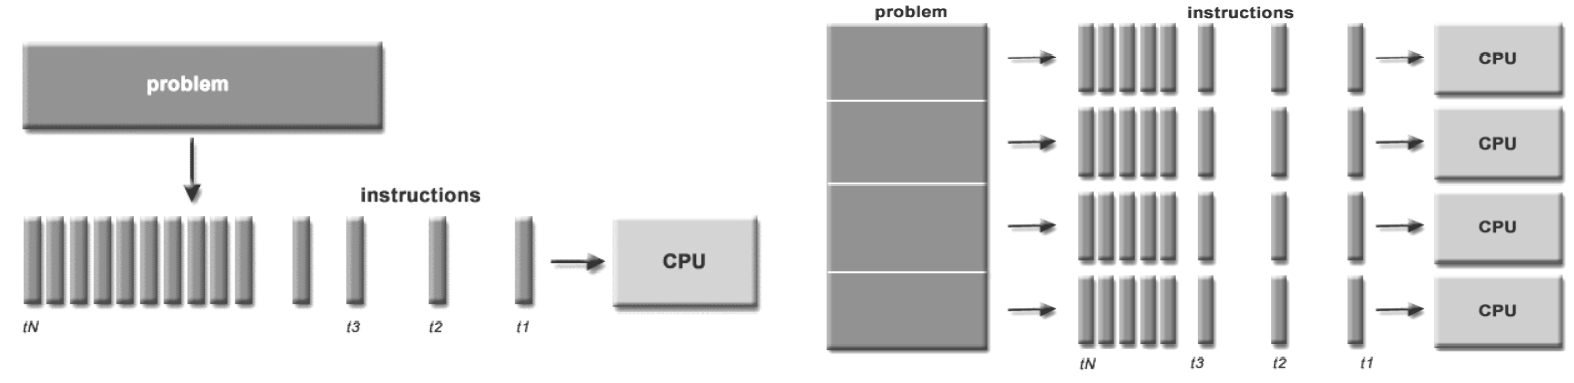
\includegraphics[width=\textwidth]{images/computacao_paralela.png}

\end{frame}

%% --------------------------------------------------------

\begin{frame}{MPI}

MPI não é necessariamente um protocolo de transmissão

\vspace{0.5cm}

Também não é iniciativa de nenhum orgão regulador
\begin{itemize}
    \item IEEE, ISO, $\ldots$
\end{itemize}

\vspace{0.5cm}

O MPI nasceu a partir de uma discussão em uma conferência científica em 1991
\begin{itemize}
    \item Se tornou o padrão para comunicação entre processos
\end{itemize}
\end{frame}

%% --------------------------------------------------------

\begin{frame}{MPI}

MPI define três coisas
\begin{enumerate}
    \item Sintaxe
    \item Semântica
    \item Métodos
\end{enumerate}

\vspace{0.5cm}

Sendo assim, existem diversas diferentes implementações de MPI
\begin{itemize}
    \item Diversas linguagens de programação
\end{itemize}
\end{frame}

%% --------------------------------------------------------

\begin{frame}{Operações padrão de MPI}

Existem 7 operações básicas para se trabalhar com MPI

\begin{enumerate}
    \item MPI\_send \textcolor{sthlmDarkBlue}{$\leftarrow$} envia uma mensagem
    \item MPI\_ssend \textcolor{sthlmDarkBlue}{$\leftarrow$} envia uma mensagem e espera o início da transmissão
    \item MPI\_bsend \textcolor{sthlmDarkBlue}{$\leftarrow$} adiciona uma mensagem para um buffer
    \item MPI\_isend \textcolor{sthlmDarkBlue}{$\leftarrow$} envia uma referência para uma mensagem
    \item MPI\_sendrecv \textcolor{sthlmDarkBlue}{$\leftarrow$} envia uma mensagem e espera a resposta
    \item MPI\_recv \textcolor{sthlmDarkBlue}{$\leftarrow$} recebe uma mensagem; bloqueia caso não exista nenhuma
    \item MPI\_irecv \textcolor{sthlmDarkBlue}{$\leftarrow$} recebe uma referência para uma mensagem
\end{enumerate}

Entretanto, existem diversos métodos avançados \href{https://github.com/iagoac/dce540/blob/main/material_apoio/mpi4.0_standards.pdf}{\beamergotobutton{Link}} 
\begin{itemize}
    \item Mais de 440 métodos (MPI 3.0)
\end{itemize}
\end{frame}

%% --------------------------------------------------------

\begin{frame}{Decomposição funcional}

O problema é decomposto em diferentes tarefas, gerando diversos programas, que serão  distribuídos por entre múltiplos processadores para execução simultânea


\centering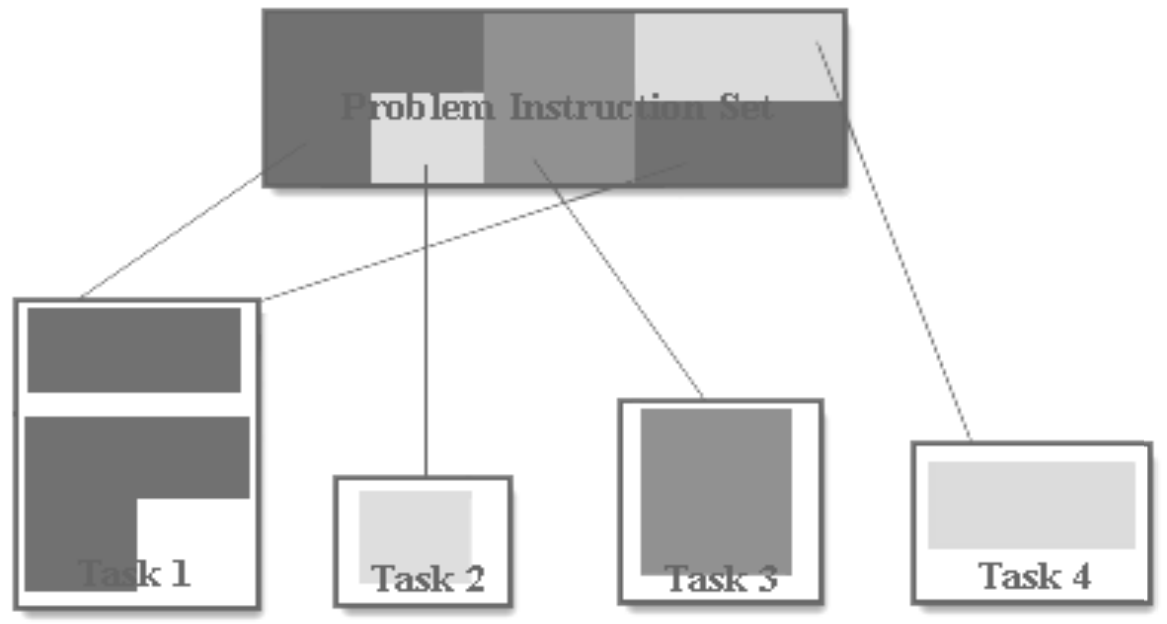
\includegraphics[width=\textwidth]{images/decomposicao_funcional.png}

\end{frame}

%% --------------------------------------------------------

\begin{frame}{Decomposição de domínio}

Os dados são decompostos em grupos, que serão distribuídos por entre múltiplos 
processadores que executarão, simultaneamente, um mesmo programa

\centering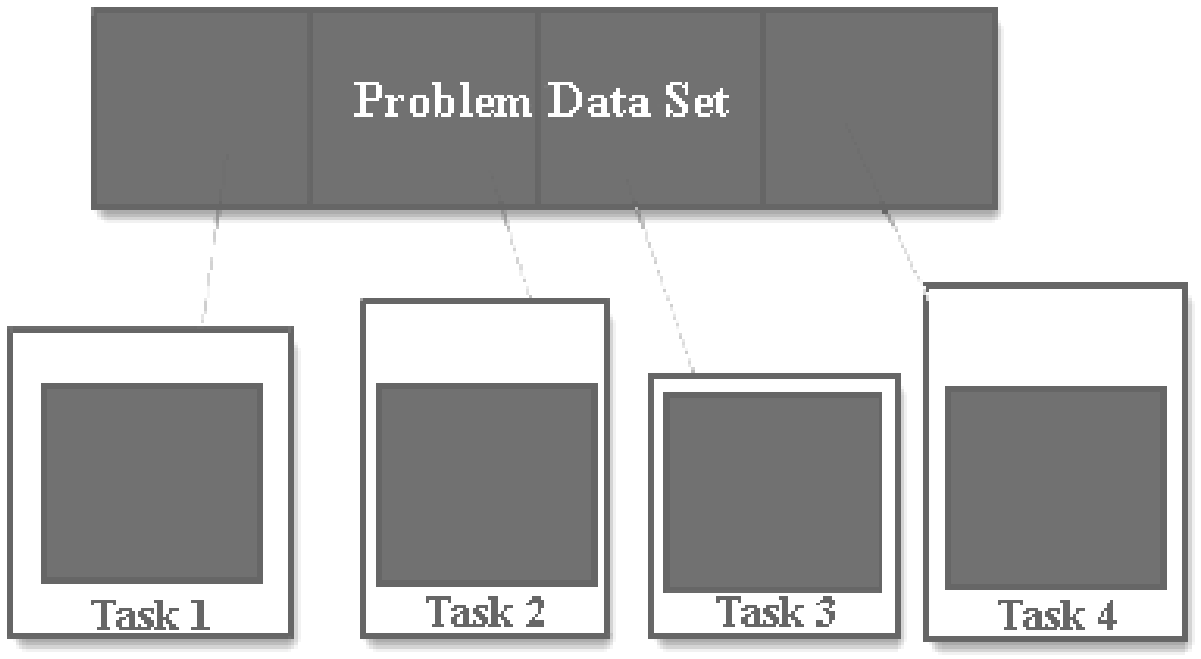
\includegraphics[width=\textwidth]{images/decomposicao_dados.png}

\end{frame}

%% --------------------------------------------------------

\begin{frame}{Speed-up e Lei de Amdahl}

\textit{Speed-up} é o nome que damos ao ganho de performance de um algoritmo ao utilizarmos computação paralela
\begin{itemize}
    \item Representa qual é o ganho de velocidade de execução de um algoritmo
\end{itemize}

\vspace{0.5cm}

No geral, o \textit{speed-up} esperado de um algoritmo pode ser calculado utilizando a Lei de Amdahl

\end{frame}

%% --------------------------------------------------------

\begin{frame}{Tempo de processamento paralelo}

$$
T(n) = T(1) \left( (1 - B) + \frac{1}{n}\,B \right),
$$

\vspace{1cm}
onde 
\begin{itemize}
    \item $n$ representa o número de threads
    \item $T(n)$ representa o tempo esperado de computação utilizando $n$ threads paralelas
    \item $B$ é a fração paralela de um algoritmo
\end{itemize}

\end{frame}

%% --------------------------------------------------------

\begin{frame}{\textit{Speed-up} teórico - Lei de Amdahl}

$$
S(n) = \frac{T(1)}{T(n)} = \frac{T(1)}{T(1) \left( (1 - B) + \frac{1}{n}\,B
\right)} = \frac{1}{ (1 - B) + \frac{1}{n}\,B}
$$

\end{frame}

%% --------------------------------------------------------

\begin{frame}{\textit{Speed-up} teórico - Lei de Amdahl}

\begin{table}[]
\centering
\resizebox{0.7\textwidth}{!}{%
\begin{tabular}{ccccc}
\hline
       & \multicolumn{4}{c}{B}      \\ \cline{2-5} 
n      & 0,25 & 0,50 & 0,75 & 0,99  \\ \hline
2      & 1,14 & 1,33 & 1,60 & 1,98  \\
10     & 1,29 & 1,82 & 3,08 & 9,17  \\
50     & 1,32 & 1,96 & 3,77 & 33,56 \\
100    & 1,33 & 1,98 & 3,88 & 50,25 \\
1000   & 1,33 & 2,00 & 3,99 & 90,99 \\
100000 & 1,33 & 2,00 & 4,00 & 99,90 \\ \hline
\end{tabular}%
}
\end{table}
\end{frame}

%% --------------------------------------------------------

\begin{frame}{\textit{Speed-up} na prática}

A Lei de Amdahl representa um limite teórico para o \textit{speed-up}

\vspace{0.5cm}

Na prática, não é bem isso o que acontece
\begin{itemize}
    \item \textit{Speed-up} é sub-linear (em relação a $n$)
    \item Tempo de barramento
    \item Tempo de acesso a memória
    \item Tempo para "juntar" as informações
\end{itemize}

\vspace{0.5cm}

Em raríssimos casos, pode acontecer um \textit{speed-up} super-linear!
\begin{itemize}
    \item Diferentes velocidades de memória cache dos processadores
\end{itemize}
\end{frame}

\end{document}
